\documentclass[border=6pt]{standalone}
\usepackage{pgfplots}
\pgfplotsset{compat=1.18}
\begin{document}
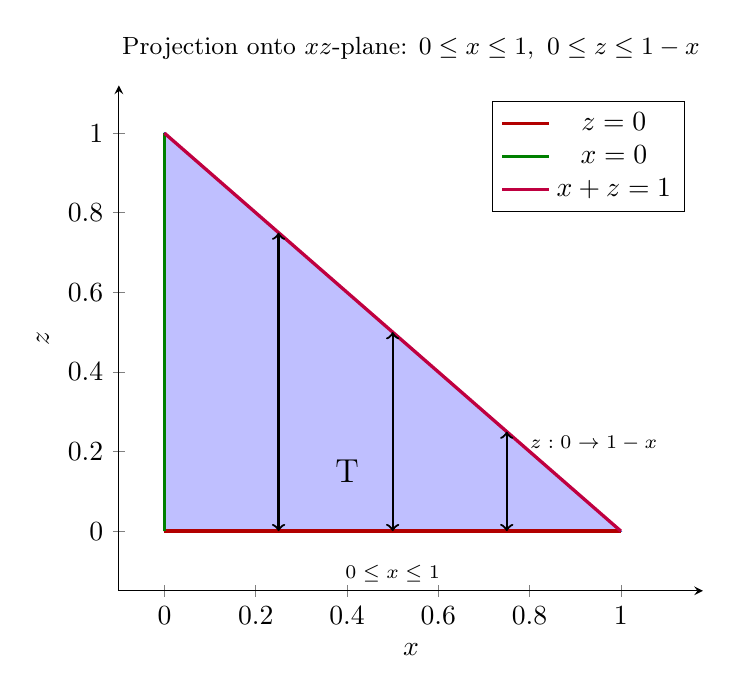
\begin{tikzpicture}
\begin{axis}[
    width=9cm, height=8cm,
    xlabel=$x$, ylabel=$z$,
    xmin=-0.1, xmax=1.18, ymin=-0.15, ymax=1.12,
    axis lines=left,
    grid=none,
    title={\small Projection onto $xz$-plane: $0\le x\le 1,\ 0\le z\le 1-x$},
    legend pos=north east,
]
% filled triangle T  (excluded from legend)
\addplot[fill=blue!25, draw=blue!60!black, forget plot]
  coordinates {(0,0) (1,0) (0,1)} -- cycle;
% boundary edges with legend
\addplot[red!70!black, very thick] coordinates {(0,0) (1,0)};
\addlegendentry{$z=0$}
\addplot[green!50!black, very thick] coordinates {(0,0) (0,1)};
\addlegendentry{$x=0$}
\addplot[purple, very thick] coordinates {(1,0) (0,1)};
\addlegendentry{$x+z=1$}
% label T
\node at (axis cs:0.4,0.15) {\large T};
% arrows indicating z-range for fixed x
\draw[<->, thick] (axis cs:0.25,0) -- (axis cs:0.25,0.75);
\draw[<->, thick] (axis cs:0.50,0) -- (axis cs:0.50,0.50);
\draw[<->, thick] (axis cs:0.75,0) -- (axis cs:0.75,0.25);
\node[anchor=west] at (axis cs:0.78,0.22) {\scriptsize $z:0\to 1-x$};
\node[anchor=north] at (axis cs:0.5,-0.06) {\scriptsize $0\le x\le 1$};
\end{axis}
\end{tikzpicture}
\end{document}
